% Draft No. 1
  % Description
  % Instructions
  % Tips and tricks
  % Grading
% Estimation
  % Central Limit Theorem
  % Law of Large Numbers
  % Confidence intervals
% Practice
  % Example: NHIS dataset
  % Practice session
  % Exercise

\documentclass[t]{beamer}
\usetheme{hkllite}

\title{estimation}
	\author{François Briatte \& Ivaylo Petev}
	\date{Week~\#5}

\begin{document}

  \frame[plain]{
		\titlepage\\[7.25em]
		\begin{columns}[T]
			\column{.4\textwidth}
				\tableofcontents[hideallsubsections]
			\column{.5\textwidth}
				\href{http://xkcd.com/385/}{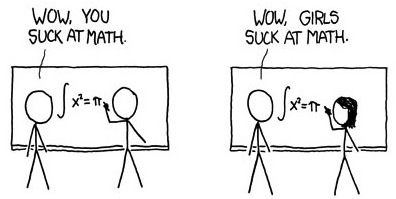
\includegraphics[width=\textwidth]{xkcd-generalization.jpg}}		
		\end{columns}
	}
	%
	%

  % %
  % %
  % \section{Draft No. 1}
  % %
  % %
  %
  % %
  % %
  % \subsection{Description}
  % %
  % %
  %
  % \begin{frame}[t]{Draft No. 1}
  %
  % \begin{columns}[T]
  %   \column{.3\textwidth}
  %
  %     \textbf{Univariate\\statistics}\\[.5em]
  %
  %     \begin{itemize}
  %       \item Introduction
  %       % (topic)
  %       \item Datasets
  %       % (observations and variables)
  %       \item Distributions
  %       % (central tendency, variability, normality)
  %       \item (Estimation)
  %       % (PDF, CLT, LLN, CIs)
  %     \end{itemize}
  %
  %     \begin{center}
  %       \red{First draft}\\[.5em]
  %       \fbox{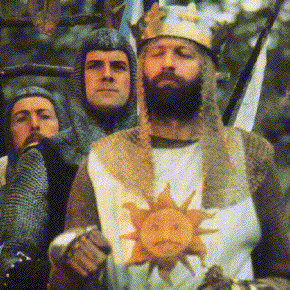
\includegraphics[width=.75\textwidth]{holy-grail2.jpg}}
  %     \end{center}
  %
  %   \column{.3\textwidth}
  %
  %     \textbf{Bivariate\\statistics}
  %
  %     \begin{itemize}
  %       \item Significance
  %       % (comparison of means and proportions)
  %       \item Comparisons
  %       % (t-test, Chi-squared test)
  %       \item Correlation
  %       % (scatterplot and correlation matrixes)
  %       \item Regression
  %       % (Simple OLS linear regression)
  %     \end{itemize}
  %
  %     \begin{center}
  %       Revised draft\\[.5em]
  %     \end{center}
  %
  %   \column{.3\textwidth}
  %
  %     \textbf{Statistical\\modelling}
  %
  %     \begin{itemize}
  %       \item Basics
  %       % (residuals)
  %       \item Extensions
  %       % (dummies)
  %       \item Diagnostics
  %       % (multicollinearity, heteroscedasticity)
  %       \item Conclusion
  %       % (extensions)
  %     \end{itemize}
  %
  %     \begin{center}
  %       Final paper\\[.5em]
  %       \fbox{
\includegraphics[width=.75\textwidth]{holy-grail.jpg}}
  %     \end{center}
  %
  % \end{columns}
  %
  % \end{frame}
  % %
  % %
  %
  % %
  % %
  % \subsection{Instructions}
  % %
  % %
  %
  % \begin{frame}[t]{Instructions}
  %
  %   \begin{block}{Catch up}
  %     \begin{itemize}
  %       \item \textbf{Readings:} Stata Guide (and handbook chapters)
  %       \item \textbf{Replication:} all do-files so far
  %       \item \textbf{Projects:} student list at \href{http://goo.gl/xNGmDA}{goo.gl/xNGmDA}
  %     \end{itemize}
  %   \end{block}
  %
  %   \begin{block}{Write up}
  %     \begin{itemize}
  %       \item \textbf{Copy} the paper template to your Google Drive
  %       \item \textbf{Share} the renamed template within your group
  %       \item \textbf{Share} the renamed template with me :)
  %     \end{itemize}
  %   \end{block}
  %
  % \end{frame}
  % %
  % %
  %
  %   % \begin{frame}[t]{\red{Common mistakes}}
  %   %
  %   %   \begin{alertblock}{Project files}
  %   %     \begin{itemize}
  %   %       \item \textbf{Filenames:} use your \red{group shortname}
  %   %       \item \textbf{Formats:} use \red{PDF} (paper) and \red{.do} (code)
  %   %       \item \textbf{ENTG:} use groups %
  %   %         \texttt{57344}, \texttt{57345} and \texttt{57346}
  %   %     \end{itemize}
  %   %   \end{alertblock}
  %   %
  %   %   \begin{alertblock}{Paper content}
  %   %     \begin{itemize}
  %   %       \item \textbf{Paragraphs:} respect limits, write analytically
  %   %       \item \textbf{Table formats:} single-paged, rounded figures
  %   %       \item \textbf{Sources:} format your bibliography, cite the data
  %   %     \end{itemize}
  %   %   \end{alertblock}
  %   %
  %   % \end{frame}
  %   % %
  %   % %
  %
  % %
  % %
  % \subsection{Tips and tricks}
  % %
  % %
  %
  % \begin{frame}[t]{Survival techniques}
  %
  %   \begin{block}{Code}
  %     \begin{itemize}
  %       \item \textbf{Copy} code chunks from the course do-files
  %       \item \textbf{Run} the code entirely to check for errors
  %       \item \textbf{Log} your results to analyze them later
  %     \end{itemize}
  %   \end{block}
  %
  %   \begin{block}{Paper}
  %     \begin{itemize}
  %       \item \textbf{Write} as the authors of the example papers
  %       \item \textbf{Hypothesize} from structural determinants to covariates
  %       \item \textbf{Select} only the statistics that you can analyze
  %     \end{itemize}
  %   \end{block}
  %
  % \end{frame}
  % %
  % %
  %
  % \begin{frame}[t]{Extra tips}
  %
  %   \begin{block}{Research tips}
  %     \begin{itemize}
  %       \item \textbf{Maximize sample size:} %
  %         keep the data representative
  %       \item \textbf{For a continuous DV,} %
  %         normality matters for linear regression
  %       \item \textbf{For a categorical DV,} %
  %         recode to binary for logistic regression
  %     \end{itemize}
  %   \end{block}
  %
  %   \begin{block}{Graph tips}
  %     \begin{itemize}
  %       \item \textbf{Keep graphs open} %
  %         with \code{name()}; leave them out of the paper
  %       \item \textbf{Plot over small multiples} %
  %         with \code{over()} and \code{by()}
  %       \item \textbf{Use the IOTT} %
  %         to decide whether to keep or ditch a graph
  %     \end{itemize}
  %   \end{block}
  %
  % \end{frame}
  % %
  % %
  %
  % %
  % %
  % \subsection{Grading}
  % %
  % %
  %
  % \begin{frame}[t]{Grading scheme}
  %
  %   \begin{block}{Protocol}
  %     \begin{enumerate}
  %       \item \textbf{Replicate findings:} %
  %         run code, open results log
  %       \item \textbf{Review design:} %
  %         check sources, hypotheses
  %       \item \textbf{Suggest improvements:} %
  %         variables, plots, references, …
  %     \end{enumerate}
  %   \end{block}
  %
  %   \begin{exampleblock}{Best papers}
  %     \begin{itemize}
  %       \item \textbf{Questions on front page}, %
  %         with line numbers for code issues
  %       \item \textbf{No spelling mistakes}, %
  %         with no formatting issues throughout
  %       \item \textbf{Selected, rounded statistics}, %
  %         all with a specific interpretation
  %     \end{itemize}
  %   \end{exampleblock}
  %
  % \end{frame}
  % %
  % %
	
	\begin{frame}[t,plain]
		
		\vspace{.3\paperwidth}
		\begin{center}
			{\Large Brace yourself for a \red{little math}.}
		\end{center}
		
		\vspace{1em}
		\begin{flushright}
			
\includegraphics[scale=.3]{longcat-white.jpg}		
		\end{flushright}

	\end{frame}
	%
	%
	
	%
	%
	\section{Estimation}
	%
	%
	
	\begin{frame}[t]{Estimation}

		\begin{block}{The issue}
			\begin{itemize}
				\item The \textbf{sample parameter} %
					is the sample mean $\bar X$
				\item The \textbf{population parameter} %
					is the population mean $\mu$
				\item How to \textbf{generalize} %
					from sample to population?
			\end{itemize}
		\end{block}
		
		\begin{block}{The solution}
			\begin{itemize}
				\item \textbf{Central Limit Theorem} (CLT)
					% $\bar X$ relates to $\mu$ via a normal distribution
				\item \textbf{Law of Large Numbers:} (LLN)
					%with no formatting issues throughout
				\item \textbf{Confidence intervals:} (CIs)
					%a range of values likely to contain $\mu$
			\end{itemize}
		\end{block}
		
	\end{frame}
	%
	%

	% 
	% 	
	\subsection{Central Limit Theorem}
	%
	%

	\begin{frame}[t]{Central Limit Theorem}

			\begin{block}{Definition}
				The independent %
				and identically distributed %
				means $\bar X_1, \bar X_2, \cdots, \bar X_n$ of %
				repeated random samples are %
				\red{normally distributed around $\mu$}.
			\end{block}

			\begin{columns}[T]
				\column{.6\textwidth}
		
					\begin{block}{Formula}
						$$\textsf{CLT}: \red{\sqrt{N}}\bigg(\frac{1}{N}\sum_{i=1}^N \bar X_i - \mu\bigg)\ \xrightarrow{d}\ \red{\mathcal{N}(0,\;\sigma^2)}$$
					\end{block}
		
				\column{.3\textwidth}

				\vspace{1em}
				\begin{flushright}
					
\includegraphics[scale=.3]{longcat-white.jpg}		
				\end{flushright}
			\end{columns}
		
	\end{frame}
	%
	%

	%
	%
	\subsection{Law of Large Numbers}
	%
	%

	\begin{frame}[t]{Law of Large Numbers}

			\begin{block}{Definition}
				The sample standard deviation $SD_x$ converges towards the population %
				standard deviation $\sigma$ at a speed of $\sqrt{N}$. 
			\end{block}

			\begin{columns}[T]
				\column{.6\textwidth}
		
					\begin{block}{Formula}
						$$\textsf{SEM} = SE_{\bar X} = \frac{SD}{\red{\sqrt{N}}}$$
					\end{block}
		
				\column{.3\textwidth}

				\vspace{1em}
				\begin{flushright}
					
\includegraphics[scale=.3]{longcat-white.jpg}		
				\end{flushright}
			\end{columns}
		
	\end{frame}
	%
	%

	\begin{frame}[t]{Standard normal distribution $\mathcal{N}(0,1)$}
	
	\begin{block}{Properties}
		\begin{itemize}
			\item $\mu \pm 1\sigma$ contains approximately \textbf{68\%} of all values.
			\item $\mu \pm 2\sigma$ contains approximately \textbf{95\%} of all values.
			\item $\mu \pm 3\sigma$ contains approximately \textbf{99\%} of all values.
		\end{itemize}
	\end{block}
	
	\begin{center}
		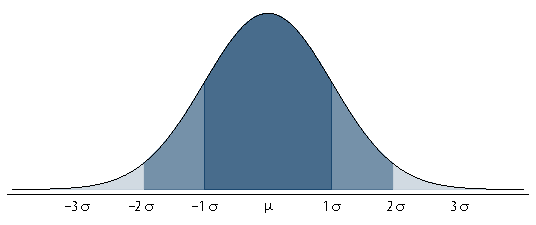
\includegraphics[width=.8\textwidth]{normal-distribution.pdf}
	\end{center}
		
	\end{frame}
	%
	%
	
	\begin{frame}[t]{Probability density function}
	
	\begin{block}{Properties}	
		\begin{itemize}
			\item $Pr(\mu - 1\sigma < \mu < \mu + 1\sigma) \approx .68$
			\item $Pr(\mu - 2\sigma < \mu < \mu + 2\sigma) \approx .95$
			\item $Pr(\mu - 3\sigma < \mu < \mu + 3\sigma) \approx .99$
		\end{itemize}
	\end{block}
	
	\begin{center}
		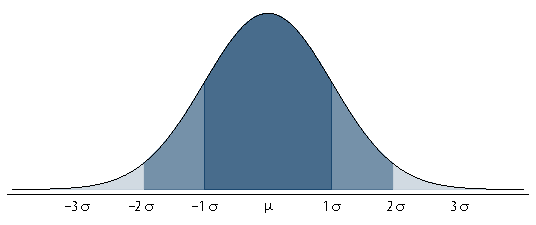
\includegraphics[width=.8\textwidth]{normal-distribution.pdf}
	\end{center}
		
	\end{frame}
	%
	%

	%
	% 	
	\subsection{Confidence intervals}
	%
	% 		
	\begin{frame}[t]{Confidence intervals}

	Given these properties, the population mean $\mu$ can be estimated from a sample $X$ of $N$ (statistically independent) observations.\vspace{1em}

%	\begin{itemize}
%		\item 
		\textbf{When we observe a normal distribution}, $\mu \pm 2\sigma$ contains approximately 95\% of all values. The exact number used for estimation at \red{95\% confidence}, called the \red{z-score}, is $z = 1.96$.\\
		\vspace{1em}
%		\item 
\textbf{When the sample values of $X$ are normally distributed}, $\bar X \pm 1.96 \cdot SE_{\bar X}$ contains 95\% of the possible values of $\mu$.\\[1em]

These bounds define a \red{95\% confidence interval}.

%	\end{itemize}

	\begin{columns}[T]
		\column{.625\textwidth}
		\hspace{.725em}
		\begin{itemize}
			\item In 2.5\% of cases, $\mu < \bar{X} - 1.96$.
			\item In 2.5\% of cases, $\mu > \bar{X} + 1.96$.
		\end{itemize}
		\column{.3\textwidth}
		\vspace{-4em}
		\begin{flushright}
		
\includegraphics[scale=.3]{longcat-white.jpg}		
		\end{flushright}
	\end{columns}
	
	\end{frame}

% 	
% 	\subsection{Back to Estimation}
% 		
% 	\begin{frame}[t]{Back to estimation}
% 	
% 	Using the normal distribution as a probability density function and standardised $z$-scores to select a level of confidence:

	%
	%
	\section{Practice}
	%	
	%

	%
	%
	\subsection{Example: NHIS dataset}
	%
	%
	
	\begin{frame}[t]{Practice: \red{NHIS dataset}}

		$$\mathsf{Body~Mass~Index} = \frac{\mbox{mass} \ \mbox{(kg)}}{\left( \mbox{height}(\mathsf{m})\right)^2} = \frac{\mbox{mass} \ \mathsf{(lb)} \times 703}{\left(\mbox{height} (\mathsf{in})\right)^2}$$
		
		\vspace{1em}

		\begin{itemize}
			\item For \textbf{normal weight} adults, $18.5 < \mathsf{BMI} < 25$.
			\item For \textbf{overweight} adults, $25 \leq \mathsf{BMI} < 30$.
			\item For \textbf{obese }adults, $\mathsf{BMI} \geq 30$.		
		\end{itemize}

		\vspace{1em}
		
    Data:
	
			\begin{columns}[c]
				\column{.725\textwidth}
				
				\begin{itemize}
					\item National Health Interview Survey (NHIS)
					\item Sample: U.S. adult population, 2009
				\end{itemize}
	
				\column{.2\textwidth}
				
\includegraphics[width=\textwidth]{logo-nhis}
			\end{columns}
	
	\end{frame}
	%
	%
	
	%
	%
	\subsection{Practice session}
  %
  %
  
	\begin{frame}[t]{Practice session}

    \begin{block}{Class}
      \comm{Get the do-file for this week.}\\
      \code{srqm\_get week5.do}\\
      
			\comm{Open to read and replicate.}\\
			\code{doedit code/week5}\\    
    \end{block}

    \begin{alertblock}{Coursework}
      \begin{itemize}
	       \item Finish the do-file and read all comments at home.
	       \item Use the do-file as a template for your first draft.
	       \item Write up your paper, following final instructions.
      \end{itemize}
    \end{alertblock}
    		
	\end{frame}
  %
  %
	
\end{document}
